%%
% Copyright (c) 2017 - 2024, Pascal Wagler;
% Copyright (c) 2014 - 2024, John MacFarlane
%
% All rights reserved.
%
% Redistribution and use in source and binary forms, with or without
% modification, are permitted provided that the following conditions
% are met:
%
% - Redistributions of source code must retain the above copyright
% notice, this list of conditions and the following disclaimer.
%
% - Redistributions in binary form must reproduce the above copyright
% notice, this list of conditions and the following disclaimer in the
% documentation and/or other materials provided with the distribution.
%
% - Neither the name of John MacFarlane nor the names of other
% contributors may be used to endorse or promote products derived
% from this software without specific prior written permission.
%
% THIS SOFTWARE IS PROVIDED BY THE COPYRIGHT HOLDERS AND CONTRIBUTORS
% "AS IS" AND ANY EXPRESS OR IMPLIED WARRANTIES, INCLUDING, BUT NOT
% LIMITED TO, THE IMPLIED WARRANTIES OF MERCHANTABILITY AND FITNESS
% FOR A PARTICULAR PURPOSE ARE DISCLAIMED. IN NO EVENT SHALL THE
% COPYRIGHT OWNER OR CONTRIBUTORS BE LIABLE FOR ANY DIRECT, INDIRECT,
% INCIDENTAL, SPECIAL, EXEMPLARY, OR CONSEQUENTIAL DAMAGES (INCLUDING,
% BUT NOT LIMITED TO, PROCUREMENT OF SUBSTITUTE GOODS OR SERVICES;
% LOSS OF USE, DATA, OR PROFITS; OR BUSINESS INTERRUPTION) HOWEVER
% CAUSED AND ON ANY THEORY OF LIABILITY, WHETHER IN CONTRACT, STRICT
% LIABILITY, OR TORT (INCLUDING NEGLIGENCE OR OTHERWISE) ARISING IN
% ANY WAY OUT OF THE USE OF THIS SOFTWARE, EVEN IF ADVISED OF THE
% POSSIBILITY OF SUCH DAMAGE.
%%

%%
% This is the Eisvogel pandoc LaTeX template.
%
% For usage information and examples visit the official GitHub page:
% https://github.com/Wandmalfarbe/pandoc-latex-template
%%

% Options for packages loaded elsewhere
\PassOptionsToPackage{unicode}{hyperref}
\PassOptionsToPackage{hyphens}{url}
\PassOptionsToPackage{dvipsnames,svgnames,x11names,table}{xcolor}
%
\documentclass[
  paper=a4,
  ,captions=tableheading
]{scrartcl}
\usepackage{amsmath,amssymb}
% Use setspace anyway because we change the default line spacing.
% The spacing is changed early to affect the titlepage and the TOC.
\usepackage{setspace}
\setstretch{1.2}
\usepackage{iftex}
\ifPDFTeX
  \usepackage[T1]{fontenc}
  \usepackage[utf8]{inputenc}
  \usepackage{textcomp} % provide euro and other symbols
\else % if luatex or xetex
  \usepackage{unicode-math} % this also loads fontspec
  \defaultfontfeatures{Scale=MatchLowercase}
  \defaultfontfeatures[\rmfamily]{Ligatures=TeX,Scale=1}
\fi
\usepackage{lmodern}
\ifPDFTeX\else
  % xetex/luatex font selection
\fi
% Use upquote if available, for straight quotes in verbatim environments
\IfFileExists{upquote.sty}{\usepackage{upquote}}{}
\IfFileExists{microtype.sty}{% use microtype if available
  \usepackage[]{microtype}
  \UseMicrotypeSet[protrusion]{basicmath} % disable protrusion for tt fonts
}{}
\makeatletter
\@ifundefined{KOMAClassName}{% if non-KOMA class
  \IfFileExists{parskip.sty}{%
    \usepackage{parskip}
  }{% else
    \setlength{\parindent}{0pt}
    \setlength{\parskip}{6pt plus 2pt minus 1pt}}
}{% if KOMA class
  \KOMAoptions{parskip=half}}
\makeatother
\usepackage{xcolor}
\definecolor{default-linkcolor}{HTML}{A50000}
\definecolor{default-filecolor}{HTML}{A50000}
\definecolor{default-citecolor}{HTML}{4077C0}
\definecolor{default-urlcolor}{HTML}{4077C0}
\usepackage[margin=2.5cm,includehead=true,includefoot=true,centering,]{geometry}
\usepackage{longtable,booktabs,array}
\usepackage{calc} % for calculating minipage widths
% Correct order of tables after \paragraph or \subparagraph
\usepackage{etoolbox}
\makeatletter
\patchcmd\longtable{\par}{\if@noskipsec\mbox{}\fi\par}{}{}
\makeatother
% Allow footnotes in longtable head/foot
\IfFileExists{footnotehyper.sty}{\usepackage{footnotehyper}}{\usepackage{footnote}}
\makesavenoteenv{longtable}
% add backlinks to footnote references, cf. https://tex.stackexchange.com/questions/302266/make-footnote-clickable-both-ways
\usepackage{footnotebackref}
\usepackage{graphicx}
\makeatletter
\newsavebox\pandoc@box
\newcommand*\pandocbounded[1]{% scales image to fit in text height/width
  \sbox\pandoc@box{#1}%
  \Gscale@div\@tempa{\textheight}{\dimexpr\ht\pandoc@box+\dp\pandoc@box\relax}%
  \Gscale@div\@tempb{\linewidth}{\wd\pandoc@box}%
  \ifdim\@tempb\p@<\@tempa\p@\let\@tempa\@tempb\fi% select the smaller of both
  \ifdim\@tempa\p@<\p@\scalebox{\@tempa}{\usebox\pandoc@box}%
  \else\usebox{\pandoc@box}%
  \fi%
}
% Set default figure placement to htbp
% Make use of float-package and set default placement for figures to H.
% The option H means 'PUT IT HERE' (as  opposed to the standard h option which means 'You may put it here if you like').
\usepackage{float}
\floatplacement{figure}{H}
\makeatother
\setlength{\emergencystretch}{3em} % prevent overfull lines
\providecommand{\tightlist}{%
  \setlength{\itemsep}{0pt}\setlength{\parskip}{0pt}}
\setcounter{secnumdepth}{-\maxdimen} % remove section numbering
\makeatletter
\@ifpackageloaded{subfig}{}{\usepackage{subfig}}
\@ifpackageloaded{caption}{}{\usepackage{caption}}
\captionsetup[subfloat]{margin=0.5em}
\AtBeginDocument{%
\renewcommand*\figurename{Figura}
\renewcommand*\tablename{Tabla}
}
\AtBeginDocument{%
\renewcommand*\listfigurename{Lista de Figuras}
\renewcommand*\listtablename{Lista de Tablas}
}
\newcounter{pandoccrossref@subfigures@footnote@counter}
\newenvironment{pandoccrossrefsubfigures}{%
\setcounter{pandoccrossref@subfigures@footnote@counter}{0}
\begin{figure}\centering%
\gdef\global@pandoccrossref@subfigures@footnotes{}%
\DeclareRobustCommand{\footnote}[1]{\footnotemark%
\stepcounter{pandoccrossref@subfigures@footnote@counter}%
\ifx\global@pandoccrossref@subfigures@footnotes\empty%
\gdef\global@pandoccrossref@subfigures@footnotes{{##1}}%
\else%
\g@addto@macro\global@pandoccrossref@subfigures@footnotes{, {##1}}%
\fi}}%
{\end{figure}%
\addtocounter{footnote}{-\value{pandoccrossref@subfigures@footnote@counter}}
\@for\f:=\global@pandoccrossref@subfigures@footnotes\do{\stepcounter{footnote}\footnotetext{\f}}%
\gdef\global@pandoccrossref@subfigures@footnotes{}}
\@ifpackageloaded{float}{}{\usepackage{float}}
\floatstyle{ruled}
\@ifundefined{c@chapter}{\newfloat{codelisting}{h}{lop}}{\newfloat{codelisting}{h}{lop}[chapter]}
\floatname{codelisting}{Listing}
\newcommand*\listoflistings{\listof{codelisting}{Listas del Documento}}
\makeatother
\usepackage{bookmark}
\IfFileExists{xurl.sty}{\usepackage{xurl}}{} % add URL line breaks if available
\urlstyle{same}
\hypersetup{
  hidelinks,
  breaklinks=true,
  pdfcreator={LaTeX via pandoc with the Eisvogel template}}
\author{}
\date{}



%%
%% added
%%


%
% for the background color of the title page
%

%
% break urls
%
\PassOptionsToPackage{hyphens}{url}

%
% When using babel or polyglossia with biblatex, loading csquotes is recommended
% to ensure that quoted texts are typeset according to the rules of your main language.
%
\usepackage{csquotes}

%
% captions
%
\definecolor{caption-color}{HTML}{777777}
\usepackage[font={stretch=1.2}, textfont={color=caption-color}, position=top, skip=4mm, labelfont=bf, singlelinecheck=false, justification=raggedright]{caption}
\setcapindent{0em}

%
% blockquote
%
\definecolor{blockquote-border}{RGB}{221,221,221}
\definecolor{blockquote-text}{RGB}{119,119,119}
\usepackage{mdframed}
\newmdenv[rightline=false,bottomline=false,topline=false,linewidth=3pt,linecolor=blockquote-border,skipabove=\parskip]{customblockquote}
\renewenvironment{quote}{\begin{customblockquote}\list{}{\rightmargin=0em\leftmargin=0em}%
\item\relax\color{blockquote-text}\ignorespaces}{\unskip\unskip\endlist\end{customblockquote}}

%
% Source Sans Pro as the default font family
% Source Code Pro for monospace text
%
% 'default' option sets the default
% font family to Source Sans Pro, not \sfdefault.
%
\ifnum 0\ifxetex 1\fi\ifluatex 1\fi=0 % if pdftex
    \usepackage[default]{sourcesanspro}
  \usepackage{sourcecodepro}
  \else % if not pdftex
    \usepackage[default]{sourcesanspro}
  \usepackage{sourcecodepro}

  % XeLaTeX specific adjustments for straight quotes: https://tex.stackexchange.com/a/354887
  % This issue is already fixed (see https://github.com/silkeh/latex-sourcecodepro/pull/5) but the
  % fix is still unreleased.
  % TODO: Remove this workaround when the new version of sourcecodepro is released on CTAN.
  \ifxetex
    \makeatletter
    \defaultfontfeatures[\ttfamily]
      { Numbers   = \sourcecodepro@figurestyle,
        Scale     = \SourceCodePro@scale,
        Extension = .otf }
    \setmonofont
      [ UprightFont    = *-\sourcecodepro@regstyle,
        ItalicFont     = *-\sourcecodepro@regstyle It,
        BoldFont       = *-\sourcecodepro@boldstyle,
        BoldItalicFont = *-\sourcecodepro@boldstyle It ]
      {SourceCodePro}
    \makeatother
  \fi
  \fi

%
% heading color
%
\definecolor{heading-color}{RGB}{40,40,40}
\addtokomafont{section}{\color{heading-color}}
% When using the classes report, scrreprt, book,
% scrbook or memoir, uncomment the following line.
%\addtokomafont{chapter}{\color{heading-color}}

%
% variables for title, author and date
%
\usepackage{titling}
\title{}
\author{}
\date{}

%
% tables
%

\definecolor{table-row-color}{HTML}{F5F5F5}
\definecolor{table-rule-color}{HTML}{999999}

%\arrayrulecolor{black!40}
\arrayrulecolor{table-rule-color}     % color of \toprule, \midrule, \bottomrule
\setlength\heavyrulewidth{0.3ex}      % thickness of \toprule, \bottomrule
\renewcommand{\arraystretch}{1.3}     % spacing (padding)


%
% remove paragraph indentation
%
\setlength{\parindent}{0pt}
\setlength{\parskip}{6pt plus 2pt minus 1pt}
\setlength{\emergencystretch}{3em}  % prevent overfull lines

%
%
% Listings
%
%


%
% header and footer
%
\usepackage[headsepline,footsepline]{scrlayer-scrpage}

\newpairofpagestyles{eisvogel-header-footer}{
  \clearpairofpagestyles
  \ihead*{}
  \chead*{}
  \ohead*{}
  \ifoot*{}
  \cfoot*{}
  \ofoot*{\thepage}
  \addtokomafont{pageheadfoot}{\upshape}
}
\pagestyle{eisvogel-header-footer}



%%
%% end added
%%

\begin{document}

%%
%% begin titlepage
%%

%%
%% end titlepage
%%



\section{Modelo de Interoperabilidad
JEP}\label{sec:modelo-de-interoperabilidad-jep}

\begin{itemize}
\tightlist
\item
  \hyperref[Introducciuxf3n]{Introducción}
\item
  \hyperref[entregables-grouping]{Entregables (Grouping)}

  \begin{itemize}
  \tightlist
  \item
    \hyperref[entg01.-soluciuxf3n-de-integraciuxf3n-jep-application-component]{ENTG01.
    Solución de Integración JEP (Application Component)}
  \item
    \hyperref[entg02.-servicios-de-integraciuxf3n-jep-application-service]{ENTG02.
    Servicios de Integración JEP (Application Service)}
  \item
    \hyperref[entg04.-nodo-integraciuxf3n-jep-node]{ENTG04. Nodo
    Integración JEP (Node)}

    \begin{itemize}
    \tightlist
    \item
      \hyperref[entg06.-contenedor-application-component]{ENTG06.
      Contenedor (Application Component)}

      \begin{itemize}
      \tightlist
      \item
        \hyperref[entg07-ux5cux253Cux5cux253Ctaskux5cux253Eux5cux253E-application-service]{ENTG07
        \textless\textless task\textgreater\textgreater{} (Application
        Service)}
      \end{itemize}
    \item
      \hyperref[entg05.-proceso-ux5cux253Cux5cux253Cworkerux5cux253Eux5cux253E-application-process]{ENTG05.
      Proceso \textless\textless worker\textgreater\textgreater{}
      (Application Process)}
    \end{itemize}
  \item
    \hyperref[entg03.-cicd-integraciuxf3n-jep-technology-service]{ENTG03.
    CI/CD Integración JEP (Technology Service)}
  \item
    \hyperref[entg04.-nodo-integraciuxf3n-jep-node-2]{ENTG04. Nodo
    Integración JEP (Node) 2}

    \begin{itemize}
    \tightlist
    \item
      \hyperref[entg06.-contenedor-application-component-2]{ENTG06.
      Contenedor (Application Component) 2}

      \begin{itemize}
      \tightlist
      \item
        \hyperref[entg07-ux5cux253Cux5cux253Ctaskux5cux253Eux5cux253E-application-service-2]{ENTG07
        \textless\textless task\textgreater\textgreater{} (Application
        Service) 2}
      \end{itemize}
    \item
      \hyperref[entg05.-proceso-ux5cux253Cux5cux253Cworkerux5cux253Eux5cux253E-application-process-2]{ENTG05.
      Proceso \textless\textless worker\textgreater\textgreater{}
      (Application Process) 2}
    \end{itemize}
  \end{itemize}
\item
  \hyperref[gestiuxf3n-integraciuxf3n-grouping]{Gestión Integración
  (Grouping)}

  \begin{itemize}
  \tightlist
  \item
    \hyperref[monitoreo-de-ssrvc-integraciuxf3n-constraint]{Monitoreo de
    (ssrvc) integración (Constraint)}
  \item
    \hyperref[requerimientos-integraciuxf3n-jep-requirement]{Requerimientos
    integración JEP (Requirement)}
  \item
    \hyperref[alcance-proyecto-integraciuxf3n-goal]{Alcance Proyecto
    Integración (Goal)}
  \item
    \hyperref[justificaciuxf3n-proyecto-integraciuxf3n-jep-driver]{Justificación
    Proyecto Integración JEP (Driver)}
  \item
    \hyperref[objeto-contractual-proyecto-jep-principle]{Objeto
    Contractual Proyecto JEP (Principle)}
  \item
    \hyperref[uso-de-infraestrucutra-tecnoluxf3gica-jep-constraint]{Uso
    de Infraestrucutra Tecnológica JEP (Constraint)}
  \end{itemize}
\item
  \hyperref[modelo-de-integraciuxf3n-jepux2c-2024.-softgic-grouping]{Modelo
  de Integración JEP, 2024. Softgic (Grouping)}

  \begin{itemize}
  \tightlist
  \item
    \hyperref[transporte-capability]{Transporte (Capability)}
  \item
    \hyperref[plano-de-administraciuxf3n-capability]{Plano de
    Administración (Capability)}
  \item
    \hyperref[esquema-de-datos-capability]{Esquema de Datos
    (Capability)}
  \item
    \hyperref[transformaciuxf3n-de-mensajes-capability]{Transformación
    de Mensajes (Capability)}
  \item
    \hyperref[modelo-de-seguridad-capability]{Modelo de Seguridad
    (Capability)}
  \item
    \hyperref[condiciones-de-despliegue-capability]{Condiciones de
    Despliegue (Capability)}
  \item
    \hyperref[composiciuxf3n-de-servicios-capability]{Composición de
    Servicios (Capability)}
  \item
    \hyperref[proveedores-y-consumidores-capability]{Proveedores y
    Consumidores (Capability)}
  \item
    \hyperref[alcance-de-la-integraciuxf3n-capability]{Alcance de la
    Integración (Capability)}
  \item
    \hyperref[tecnologuxedas-capability]{Tecnologías (Capability)}
  \item
    \hyperref[conectividad-api-capability]{Conectividad API
    (Capability)}
  \item
    \hyperref[contratos-de-interoperabilidad-capability]{Contratos de
    Interoperabilidad (Capability)}
  \item
    \hyperref[tipo-de-comunicaciuxf3n-capability]{Tipo de Comunicación
    (Capability)}
  \item
    \hyperref[sistema-de-mensajes-capability]{Sistema de Mensajes
    (Capability)}
  \item
    \hyperref[patruxf3n-de-integraciuxf3n-eip-capability]{Patrón de
    Integración (EIP) (Capability)}
  \item
    \hyperref[integraciuxf3n-de-procesos-capability]{Integración de
    Procesos (Capability)}
  \item
    \hyperref[flujo-de-datos-capability]{Flujo de datos (Capability)}
  \item
    \hyperref[soluciuxf3n-de-integraciuxf3n-capability]{Solución de
    Integración (Capability)}
  \item
    \hyperref[ambientes-y-herramientas-capability]{Ambientes y
    Herramientas (Capability)}
  \end{itemize}
\end{itemize}

\subsection{Introducción}\label{sec:introducciuxf3n}

\begin{figure}
\centering
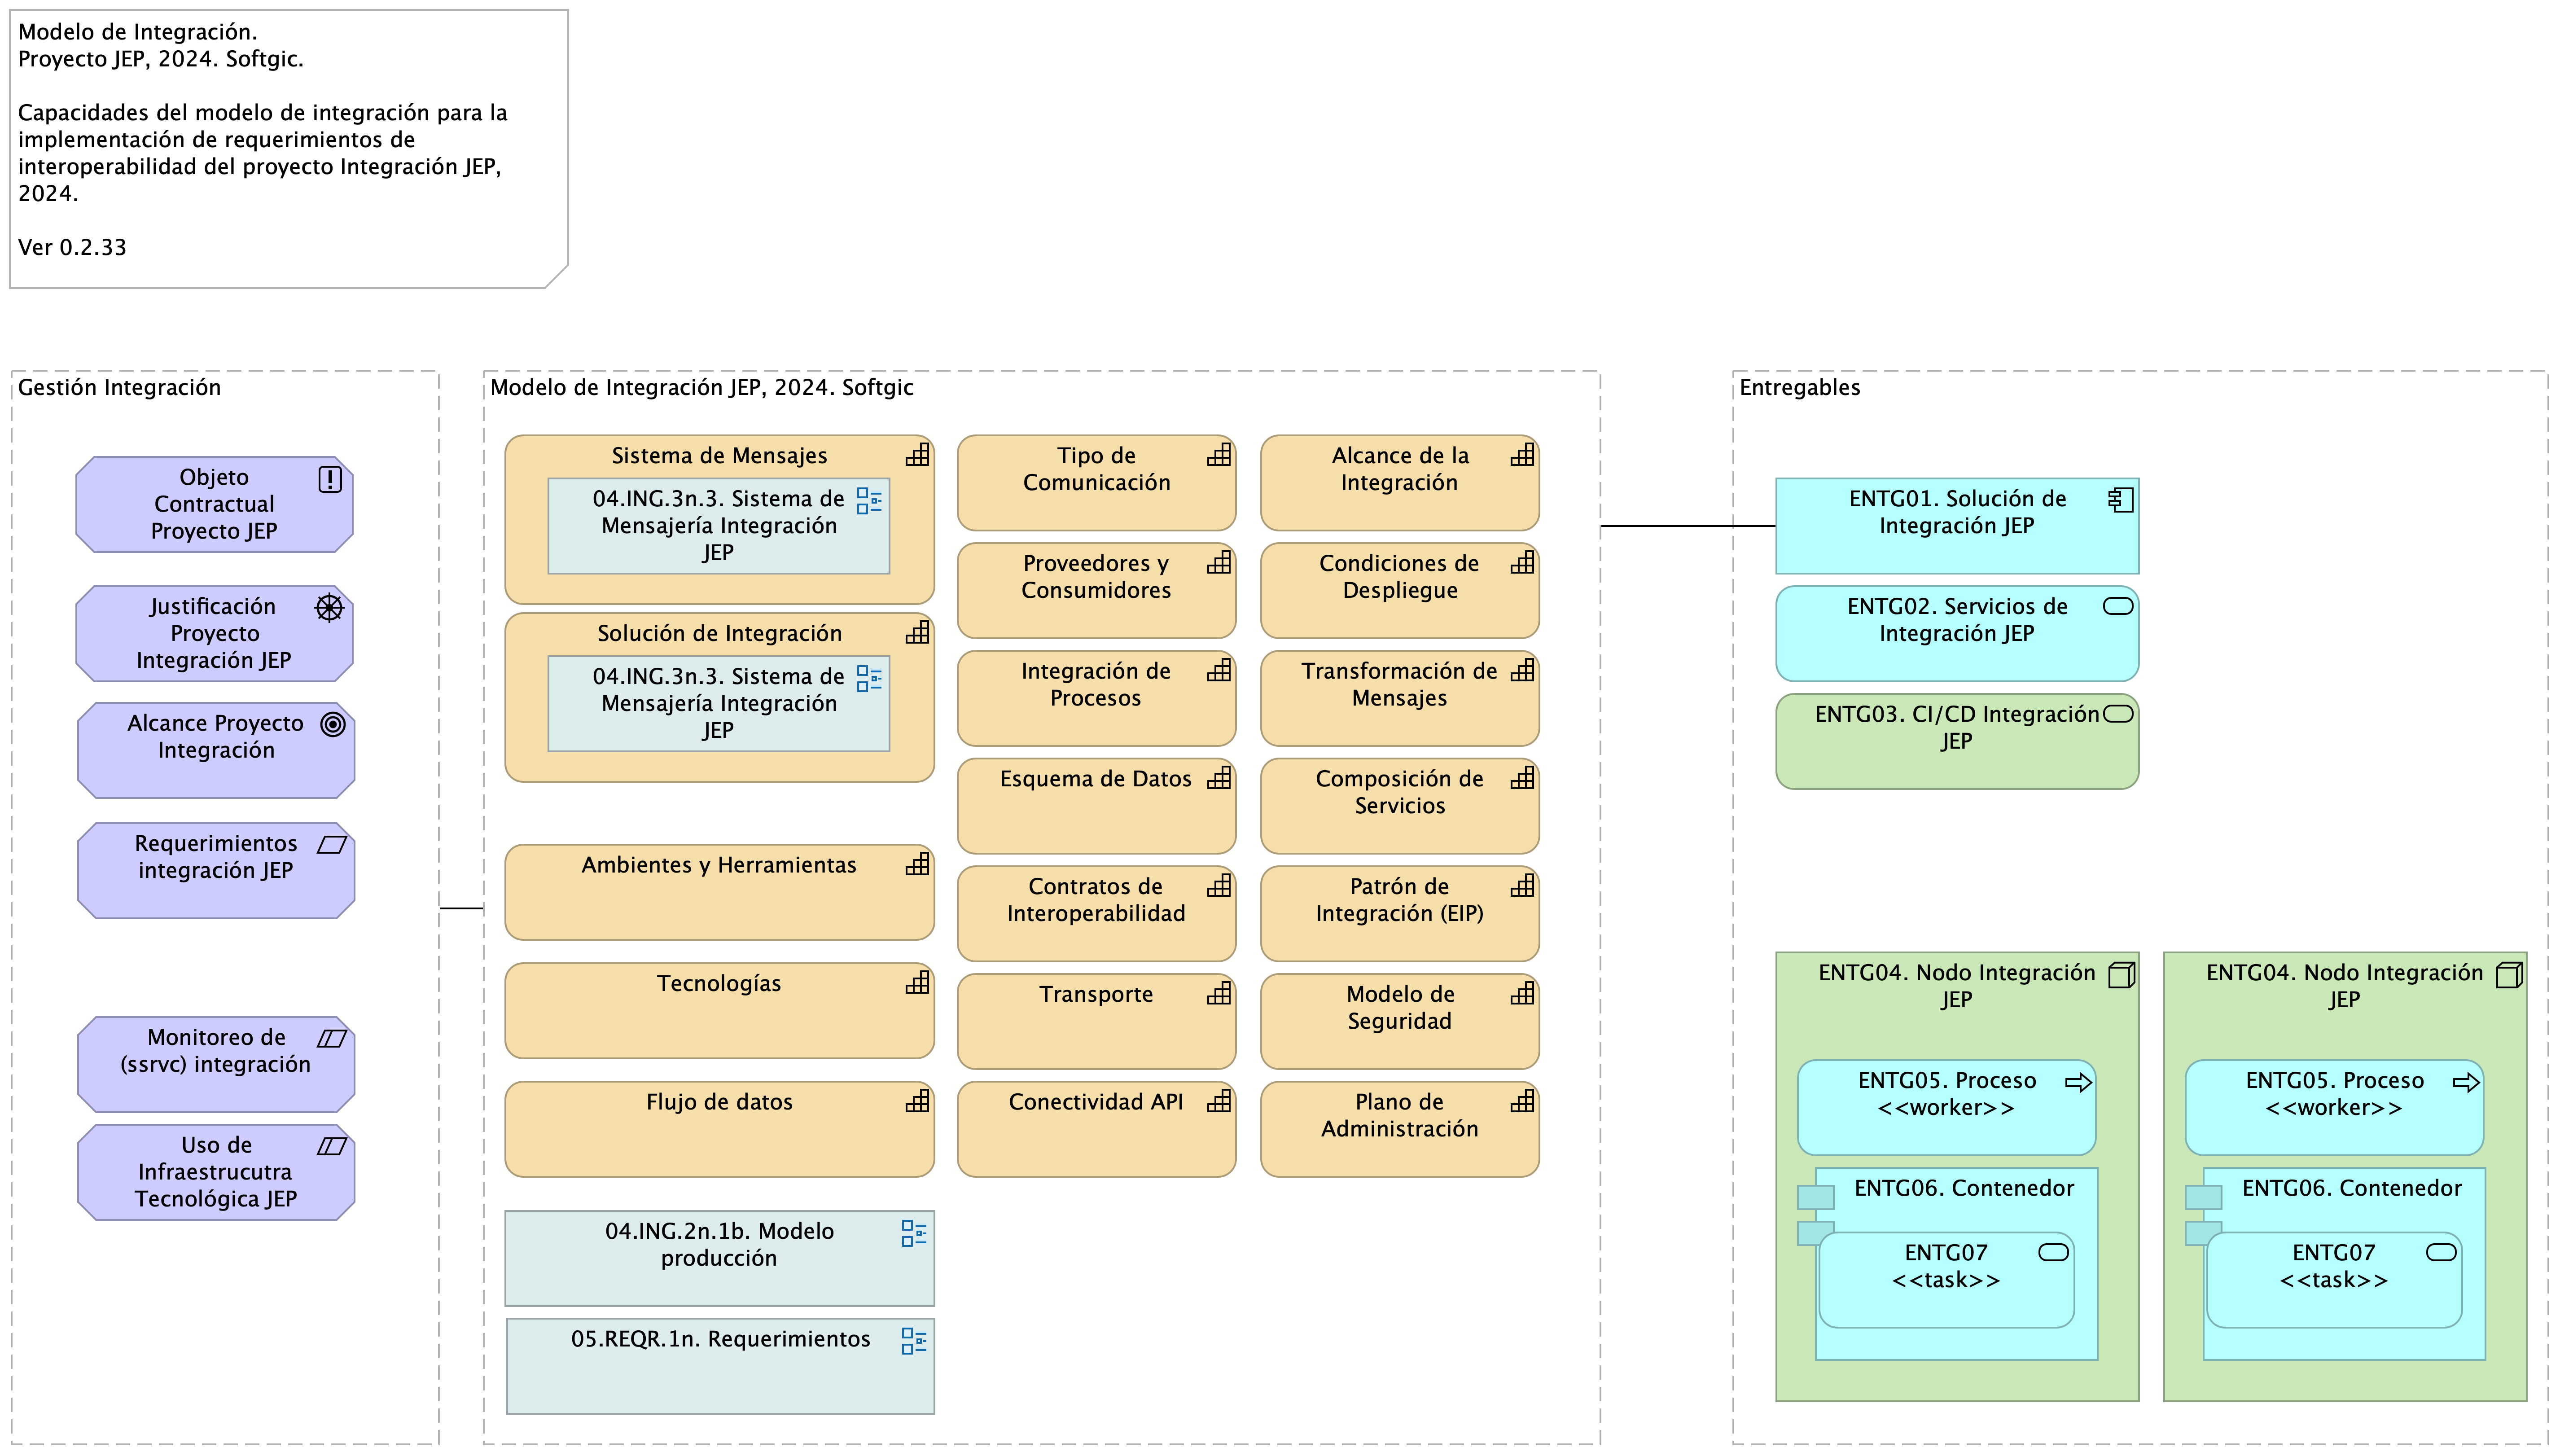
\includegraphics[width=\textwidth,height=5.20833in]{03.1n.modelointegrac.png}
\caption{04.ING.3n.1. Modelo de Interoperabilidad JEP}
\end{figure}

El presente modelo de solución de interoperabilidad JEP, 2024, en
desarrollo por Softgic, expone para aprobación y referencia las
decisiones de la solución de integración y las restricciones que la
rigen. Una vez revisado y aprobado por parte de JEP el modelo de
interoperabilidad será referencia para la gestión del proyecto y de los
entregables de esta solución.

\subsection{Características Principales del Modelo de Integración
JEP}\label{sec:caracteruxedsticas-principales-del-modelo-de-integraciuxf3n-jep}

\begin{itemize}
\tightlist
\item
  API de integración
\item
  Patrones de integración empresarial (EIP)
\item
  Sistema de Mensajería entre servicios de integración y aplicaciones
  JEP
\item
  Flujos de datos para integración
\item
  Arquitectura de clusters y contenedores para integración
\item
  Uso de infraestructura tecnológica JEP
\end{itemize}

\subsection{Entregables}\label{sec:entregables}

\subsubsection{ENTG01. Solución de Integración
JEP}\label{sec:entg01.-soluciuxf3n-de-integraciuxf3n-jep}

Documentación técnica del diseño de solución de la integración JEP,
2024.

\subsubsection{ENTG02. Servicios de Integración
JEP}\label{sec:entg02.-servicios-de-integraciuxf3n-jep}

Servicios ejecutables desplegados en los entornos de software JEP.

\subsubsection{ENTG04. Nodo Integración
JEP}\label{sec:entg04.-nodo-integraciuxf3n-jep}

Cluster de ejecución de los nodos y procesos de (servicios) de
integración del proyecto.

\paragraph{ENTG06. Contenedor}\label{sec:entg06.-contenedor}

Contenedores de los servicios de integración del proyecto desplegados en
la infraestructura tecnológica JEP.

\#\#\#\#\# ENTG07 \textless{}

\begin{quote}
\end{quote}

Servicios de integración del proyecto desplegados en la infraestructura
tecnológica JEP.

\paragraph{\texorpdfstring{ENTG05. Proceso
\textless{}\textgreater{}}{ENTG05. Proceso \textless\textgreater{}}}\label{sec:entg05.-proceso}

Configuración de servicios de integración del proyecto dentro de la
infraestructura tecnológica JEP.

\subsubsection{ENTG03. CI/CD Integración
JEP}\label{sec:entg03.-cicd-integraciuxf3n-jep}

Cadenas de integración y despliegue continuo de los servicios de
integración del proyecto de integración JEP, 2024.

\subsubsection{ENTG04. Nodo Integración
JEP}\label{sec:entg04.-nodo-integraciuxf3n-jep-1}

Cluster de ejecución de los nodos y procesos de (servicios) de
integración del proyecto.

\paragraph{ENTG06. Contenedor}\label{sec:entg06.-contenedor-1}

Contenedores de los servicios de integración del proyecto desplegados en
la infraestructura tecnológica JEP.

\#\#\#\#\# ENTG07 \textless{}

\begin{quote}
\end{quote}

Servicios de integración del proyecto desplegados en la infraestructura
tecnológica JEP.

\paragraph{\texorpdfstring{ENTG05. Proceso
\textless{}\textgreater{}}{ENTG05. Proceso \textless\textgreater{}}}\label{sec:entg05.-proceso-1}

Configuración de servicios de integración del proyecto dentro de la
infraestructura tecnológica JEP.

\subsection{Gestión Integración}\label{sec:gestiuxf3n-integraciuxf3n}

\subsubsection{Monitoreo de (ssrvc)
integración}\label{sec:monitoreo-de-ssrvc-integraciuxf3n}

\begin{itemize}
\item
  Herramientas de monitoreo y logging con las que cuenta la solución
  actual de orquestación de contenedores de OpenShift.
\item
  Monitoreo de uso de los recursos de procesamiento, red y memoria de
  los componentes claves de la solución haciendo uso de ServiceMesh.
\item
  La solución soporta la habilitación de reglas de alertas sobre los
  registros de actividad y monitoreo.
\item
  Soluciones de EFK (Elasticsearch, FluentD, Kibana - ELKstack), a
  través de operadores para centralizar el proceso de logs que se
  generan en difrerentes espacios de trabajo.
\end{itemize}

\subsubsection{Requerimientos integración
JEP}\label{sec:requerimientos-integraciuxf3n-jep}

Del alcance del proyecto 1. Implementación de 20 o más servicios de
integración al 31 de diciembre del 2024. 1. Soporte solución de
integración a julio 2025.

En donde el componente no. 1 del alcance es

\begin{itemize}
\tightlist
\item
  Desarrollar úncamente nuevos servicios de integración con el patrón de
  integración empresarial (ESB, Camel)
\item
  Implementar las condiciones tecnológicas JEP, entendido como
  requerimientos no funcionales de arquitectura, a la solución de
  integración del Anexo Nro. 1.1 -- Anexo técnico evolución plataforma
  de interoperabilidad -- Ficha Técnica
\end{itemize}

No es del alcance de este proyecto los requerimientos de migrar los
servicios existentes de modelo integración directa (EIA) esta solución
de integración empresarial.

\subsubsection{Alcance Proyecto
Integración}\label{sec:alcance-proyecto-integraciuxf3n}

\begin{itemize}
\tightlist
\item
  Implementación de 20 o más servicios de integración al 31 de diciembre
  del 2024.
\item
  Soporte solución de integración a julio 2025.
\end{itemize}

\subsubsection{Justificación Proyecto Integración
JEP}\label{sec:justificaciuxf3n-proyecto-integraciuxf3n-jep}

Justificación Proyecto Integración JEP \textbar{} Driver \textbar{}
Justification: Evolución de la Plataforma de Interoperabilidad para el
ano 2024

\begin{enumerate}
\def\labelenumi{\arabic{enumi}.}
\tightlist
\item
  Evolución de la plataforma tecnología de su interoperabilidad y el
  cumplimiento de los lineamientos del MinTIC, a traves del ``Manual
  Interactivo de Gobierno Digital, herramienta dirigida a las entidades
  publicas nacionales y territoriales (\ldots) Política de Gobierno
  Digital, Decreto 767 de 2022''
\item
  Interoperabilidad con las entidades externas que demandan información
  de la JEP
\item
  Evolución del modelo de interoperabilidad interna y gobierno de data
  maestra entre sistemas internos
\end{enumerate}

\subsubsection{Objeto Contractual Proyecto
JEP}\label{sec:objeto-contractual-proyecto-jep}

Prestar los servicios de administración y monitoreo de la solución de
interoperabilidad de los sistemas de información de la JEP; así como la
implementación de nuevos desarrollos o parametrizaciones que esta
solución requiera.

\subsubsection{Uso de Infraestrucutra Tecnológica
JEP}\label{sec:uso-de-infraestrucutra-tecnoluxf3gica-jep}

Servivios de infraestrucgtura, almacenamiento y ceomputo de la JEP:
Openshift Platform, bus empresarial, seguridad de la empresa,
tecnoglogía de clusters y contenedores.

\subsection{Modelo de Integración JEP, 2024.
Softgic}\label{sec:modelo-de-integraciuxf3n-jep-2024.-softgic}

\subsubsection{Plano de
Administración}\label{sec:plano-de-administraciuxf3n}

Monitoreo de rendimiento de ssvc de integración.

\subsubsection{Transformación de
Mensajes}\label{sec:transformaciuxf3n-de-mensajes}

Mapeos, homologaciones y correspondencias.

\subsubsection{Modelo de Seguridad}\label{sec:modelo-de-seguridad}

Autenticación mixta: JWS y tradicional (usuario, contraseña).

\subsubsection{Composición de
Servicios}\label{sec:composiciuxf3n-de-servicios}

Combina colección de servicios para formar un servicio completo.
Mediante la integración basada en patrones de Camel, define funciones
mediante la recopilación de datos de múltiples conexiones (endpoint).
Las composiciones suelen resolver integraciones no triviales o
complejas.

\subsubsection{Alcance de la
Integración}\label{sec:alcance-de-la-integraciuxf3n}

Aplicaciones que tienen integraciones existentes: necesitamos listados
de ssvc pasar al bus.

\subsubsection{Tecnologías}\label{sec:tecnologuxedas}

\begin{itemize}
\tightlist
\item
  Red Hat Integration: suite de runtimes, frameworks, y servicios para
  aplicaciones nativas de Red Hat OpenShift.
\item
  Camel Integration Tool
\item
  Quarkus development framework
\item
  Java OpenJDK 17
\item
  EFK (Elasticsearch, FluentD, Kibana - ELKstack)
\end{itemize}

\subsubsection{Conectividad API}\label{sec:conectividad-api}

Esta solución de interoperabilidad usa conectividad API REST provista
por la infraestructura de conectividad de la JEP (Apache Camel).

\subsubsection{Tipo de Comunicación}\label{sec:tipo-de-comunicaciuxf3n}

Pasar llamadas síncronas a asincrónicas: analizar apps que deben cambiar
comunicación

\subsubsection{Sistema de Mensajes}\label{sec:sistema-de-mensajes}

Esta solución de interoperabilidad usa un sistema de mensajes
(comandos). Los mensajes son de tipo petición, respuesta o excepción.

La mensajería puede ser asíncrona o síncrona entre aplicaciones o
servicios desacoplados. La conexión y la sesión es manejada por un
agente intermediario, que puede ser una cola o un bus empresarial (para
este contexto, OpenShift, Cliente Red Had Interoperabity o Apache
Camel).

La comunicación del sistema de mensajería ocurre cuando la aplicación o
servicio productor emite un comando (mensaje ) de `envío', en el cual
transmite datos o peticiones de negocio en un formato predefinido, y lo
envía a una cola de mensajes.

\subsubsection{Patrón de Integración
(EIP)}\label{sec:patruxf3n-de-integraciuxf3n-eip}

Pasar de modelo integración EIA (intgración directa ente consumidores y
proveedores) a modelo de integración EIP (integración empresarial/bus)
sobre Red Hat Integration Platform.

\subsubsection{Flujo de datos}\label{sec:flujo-de-datos}

Esta solución de interoperabilidad usa esquemas de datos predefinidos
entre las integraciones.

\subsubsection{Solución de
Integración}\label{sec:soluciuxf3n-de-integraciuxf3n}

Estilos de Integración: Communications backbone \footnote{Red troncal de
  comunicaciones: a medida que más y más aplicaciones de una empresa se
  conectan al sistema de mensajería y hacen que su funcionalidad esté
  disponible a través de la mensajería, el sistema de mensajería se
  convierte en un punto centralizado de ventanilla única para la
  funcionalidad en la empresa. Una nueva aplicación simplemente necesita
  saber qué canales usar para solicitar funcionalidad y cuáles otros
  escuchar para obtener los resultados. El propio sistema de mensajería
  se convierte esencialmente en un bus de mensajes, una columna
  vertebral que proporciona acceso a todas las diversas y cambiantes
  aplicaciones y funcionalidades de la empresa. Puedes lograr este
  nirvana de integración más rápida y fácilmente si diseñas
  específicamente para ello desde el principio.}. Patrón principal:
Messaging --- Cada aplicación (app) conectada a un mismo sistema de
mensajería, intercambio de datos y operación entre aplicaciones mediante
mensajes.

\subsubsection{Ambientes y
Herramientas}\label{sec:ambientes-y-herramientas}

Esta solución de interoperabilidad usa las herramientas, librerías,
ambientes, infraestructura productivo y no productivos (nodos, redes,
almacenamientos, y otros) indicados por la JEP.

\end{document}
